\chapter{Algorithms for Structural Variation Detection}\label{chap_related_work}

In Chapter~\ref{chap_background}, we described the biological impact of SVs, and the development of short-read sequencing technology, along with the computational challenges they represent. In this chapter we review existing algorithms for SV detection based on short-read sequencing data. We will discuss the four major computational strategies for SV detection from sequencing data, and review specific approaches, with an emphasis on algorithms that use paired sequencing reads as a primary source of information. Finally, as a demonstration of how SV detection can fit into the pipeline models we described in Chapter~\ref{chap_background}, we will describe a small pipeline for SV detection that we developed that used an existing tool, BreakDancer, to characterize SVs in a low-coverage cancer sample. 

\section{The Four Signals of SVs in Sequencing Data}

Most popular SV detection algorithms can be placed into one of four categories based on the type of signal they extract and analyze from sequencing data sets~\cite{Alkan:2011p547,Koboldt:2012gj}. The first three categories depend upon first aligning short reads to the reference genome. In Section~\ref{section_sequencing}, we described paired-end sequencing, in which both ends of a single DNA fragments are sequenced. Read pair (RP) based methods use the distance between and orientation of the mappings of these sequenced ends to identify the signatures of SVs. Out of all SV detection techniques, RP approaches are the most commonly used based on their ability to detect many types of SVs and their computational tractability~\cite{Alkan:2011p547}. Read depth (RD) approaches identify regions of the genome with anomalous coverage by read mappings, which may indicate the presence of deletions or duplications, a subcategory of SV known as copy number variations (CNVs). Split Read (SR) approaches attempt to find local mappings of portions of individual reads that span SV breakpoints. Finally, assembly-based methods attempt to construct as much of the genome sequence as possible directly from the reads, without first mapping them to the reference genome. The constructed sequence is then compared to the reference to identify SVs. Beyond these four categories, several recent approaches have attempted to integrate more than one type of signal to increase accuracy. In this review of published algorithms, we will focus on those that are built to handle whole-genome DNA resequencing from a single sample at a time; there are of course other approaches for different applications, including SV detection from targeted resequencing data such as exome sequencing, and approaches which are designed only to operate on many samples at once.

\section{Read Pair Approaches}\label{section_read_pair}

Given correct mappings of paired reads to the reference genome and a reliable estimate of the length of the fragments from which the reads came, it is relatively straightforward to detect SVs. For example, Figure~\ref{rp_signatures} shows the signatures of insertions and deletions based on the insert size of paired-end mappings: deletions lead to a longer distance between read mappings than expected, insertions to a shorter distance. Similarly, because protocols determine the orientation in which the read will be sequenced, inversions can be detected if they diverge from expectations. Finally, inversions can be detected if the reads map to different chromosomes in the reference genome. These ideas were first applied to high-throughput short-read sequencing data by Korbel et al.~\cite{Korbel:2007p544} and Campbell et al.~\cite{Campbell:2008p539}, who built upon strategies developed for analyzing SVs through the mapping of sequenced ends of larger DNA fragments (bacterial artificial chromosomes (BACs) and fosmids) from non-high-throughput sequencing data~\cite{Volik:2003fh,Raphael:2003ug,Tuzun:2005bp}.

\begin{figure}
\centering

\includegraphics[width=\textwidth]{figures/rp_signatures.pdf}
\caption[Detecting deletions and insertions from the distance between mappings of paired reads.]{Detecting deletions and insertions from the distance between mappings of paired reads. For the case of a deletion, a fragment with a 310bp internal insert size is created from the sample DNA, in a region in which 250bp has been deleted relative to the reference. The two reads when mapped to the reference will be 460bp apart, providing evidence for a deletion if we expect the internal insert size to be approximately 300bp. A 310bp internal insert size fragment that overlaps a 150bp insertion in the sample, conversely, will give a distance between reads of 180bp when mapped to the reference.}
\label{rp_signatures}
\end{figure}

Most read pair approaches use a basic strategy outlined in Figure~\ref{rp_method_workflow}. They begin by separating paired end mappings onto the reference genome into those that are \emph{concordant} and those that are \emph{discordant}, i.e. those which deviate from the expected insert size or orientation of the library. With only a few exceptions, discussed below, RP approaches discard concordant pairs and consider only discordant pairs for the remainder of their analysis. The next step is then to cluster the discordant mappings such that each cluster coherently supports a single candidate SV call. Finally, they filter or rank the candidate SV calls, for example only keeping those with support from multiple discordantly mapped read pairs. 

The BreakDancerMax component of BreakDancer~\cite{Chen:2009p3} is probably the most widely used of these algorithms\footnote{Based on a sampling of Google Scholar citation counts as of 12/28/2013: BreakDancer, 270; VariationHunter, 153; PEMer, 111; GASV, 65; SVDetect, 46.}. As described above, BreakDancer first searches for discordant read pairs based on a hard threshold on the distance between mapped paired reads. It then looks for regions of the genome that anchor more discordant read pairs than expected according to its model; if two of these regions are connected by a minimum number of discordant read pairs, it calls an SV that links them. It calls breakpoints based on the inner boundaries of the two connected regions, as illustrated in Figure~\ref{rp_method_workflow} (d), and then assigns a confidence score by computing the likelihood of the SV based on a null model in which discordant read pairs are distributed across the genome according to a mixture Poisson model. Other seminal RP-based tools include GASV~\cite{Sindi:2009gu}, PEMer~\cite{Korbel:2009dy}, VariationHunter~\cite{Hormozdiari:2009p284}, HYDRA~\cite{Quinlan:2010gf}, and SVDetect~\cite{Zeitouni:2010p8}. These all operate on similar principles, differing primarily in the method used to cluster discordant read pairs that support the same potential SV call, and in the filtering steps used to select candidate SV calls. For example, GASV formulates the clustering step in terms of a geometric model in which the goal is to find the intersection of the coordinates of breakpoints that each discordant read pair could possibly support. Marschall et al.~\cite{Marschall:2012ek} insightfully observed that most of the popular clustering procedures are computationally equivalent to solving some variant of the problem of finding maximum cliques in a graph structure in which nodes are read pairs, and edges exist if the pairs could possibly support the same variant. VariationHunter and HYDRA were also the first approaches to also integrate ambiguously mapped discordant read pairs, a topic we will consider in the next section.

Read pair approaches have the advantage of being theoretically able to detect any type of SV except for multiple copy number duplications. Their disadvantages stem from the fact that they depend on comparing mapping distances between reads to the unknown size of the fragments from which they came. This means that they cannot capture the breakpoints of SVs with single nucleotide resolution, and that they depend on having a sequencing library with a tight distribution of fragment sizes in order to have power. In addition, the fact that many SV breakpoints occur in regions with high sequence similarity to other parts of the genome, as discussed in Section~\ref{section_sv_mechanisms}, means that it may be difficult to unambiguously map reads to those locations.

\begin{figure}
\centering
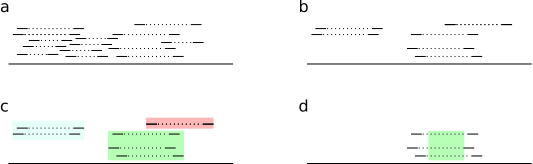
\includegraphics[width=\textwidth]{figures/rp_method_workflow.pdf}
\caption[The general algorithmic steps of a classic read-pair algorithm.]{The general algorithmic steps of a classic read-pair algorithm. a) The algorithm accepts a set of alignments of paired reads to the reference as input. b) The algorithm identifies discordant read pairs. c) Discordant pairs are clustered to find groups that could support the same algorithm. d) Clusters of discordant read pairs are filtered (in this case, by the number of supporting read pairs), and bounds on the potential breakpoints are identified.}
\label{rp_method_workflow}
\end{figure}

\subsection{Ambiguously Mapped Read Pairs}

Many of these approaches use only reads that are unambiguously mapped to the reference genome; this has the advantage of using the same set of alignments that are used for calling SNVs and indels in most sequencing pipelines. A second group of RP methods attempt to include discordant read pairs which cannot be unambiguously mapped to the reference genome in their analysis, in an effort to improve sensitivity in repetitive regions of the genome. One approach to incorporating this type of information can be found in \emph{soft clustering} algorithms, which assign each ambiguously mapped read pair to one of its mappings such that it clusters with other discordant read pairs. These approaches include VariationHunter~\cite{Hormozdiari:2009p284}, which allocates ambiguously mapped reads by optimizing a maximum parsimony explanation of all discordant reads; HYDRA~\cite{Quinlan:2010gf}, which takes a similar approach based on heuristics; and GASVPro~\cite{Sindi:2012kk}, which uses a Markov-Chain Monte Carlo sampling strategy to assign a read to its correct mapping. Even though they do consider more information than methods solely based on concordant reads, most methods in this category (with the exception of VariationHunter) use only a limited number of ambiguous discordant mappings per read pair, in part because of the storage and computational requirements necessary to process all or most ambiguous mappings of each read pair in a high-coverage data set. In Chapters~\ref{chap_cloudbreak_impl} and \ref{chap_cloudbreak_eval}, we will show that the MapReduce distributed computing framework has the potential to help address these challenges.

\subsection{Concordant Read Pairs}\label{section_mixture_of_distributions}

The RP approaches listed above only consider the mapped insert sizes of discordant read pairs. (GASVPro does consider some concordant mappings in its final output, which we will mention in Section~\ref{section_hybrid_approaches}, but only in the sense of computing an RD signal rather than actually considering the insert sizes of the concordant pairs themselves.) Since discordant read pairs make up only a very small fraction of the mapped reads in a typical sequencing data set, these approaches are not considering much of the data available. Several algorithms have tried to use the information present in concordant read pairs to generate SV predictions. One simple example can be found in ChopSticks~\cite{Yasuda:2012ij}, which refines the breakpoint locations of deletion calls based on discordant pairs by looking for concordant pairs that overlap the ends of the predicted variant. This approach only works for homozygous deletions, however, and is therefore limited in scope.

More comprehensive attempts to include concordant RP information were described in MoDIL~\cite{Lee:2009da} and the BreakDancerMini component of BreakDancer~\cite{Chen:2009p3}. MoDIL models the distribution of insert sizes at candidate locations in the genome using a Gaussian mixture model (GMM) describing the insert sizes observed; deletions and insertions are represented as additional components in the mixture. This has two advantages: because reads are not categorized as concordant or discordant based on a hard threshold, it is possible to detect smaller insertions and deletions; and these approaches can explicitly model the zygosity (presence of the variant on one or both of the pairs of chromosomes in the cell) of the variant in the sample, and potentially classify the variant as homozygous or heterozygous. The disadvantage of this approach in these implementations has been the computational requirements. BreakDancerMini considered \emph{only} concordant read pairs, after processing discordant pairs in the BreakDancerMax. For each location in the genome they executed a sliding window Kolmogorov-Smirnov test comparing the distribution of concordant insert sizes to that of the entire library. This limited the approach to detecting only very small variants; the authors of BreakDancer no longer recommend running BreakDancerMini, presumably because of its computational requirements, instead suggesting SR-based approaches such as Pindel~\cite{Ye:2009p2} to find smaller insertion and deletion variants. In Chapters~\ref{chap_cloudbreak_impl} and \ref{chap_cloudbreak_eval}, we will show that a strategy that considers the RP signal present in concordant read pairs can be made to give highly accurate result with very fast runtimes through the use of an algorithm developed in the MapReduce distributed computing framework.

Finally, CLEVER~\cite{Marschall:2012ek} took an alternative approach based on constructing a graph linking all paired reads, both concordant and discordant, that could support the same allele at a position, and then clustering reads based on finding maximum cliques in the graph. As mentioned above, they showed that this is conceptually similar to the clustering approaches used by other algorithms for discordant reads. They demonstrated that their approach was superior at detecting smaller variants because of its lack of hard thresholds for discordancy, and provided a relatively efficient implementation that can process a full 30X genome in approximately 8 hours.

\section{Read Depth Approaches}

Read-depth (RD) approaches consider the changing depth of coverage of concordantly mapped reads along the genome to infer the presence of SVs. For example, a homozygously deleted region will have zero coverage in the reference genome, while a region that has been duplicated many times, as can happen in some regions of the genome and in some cancers, will have a much higher coverage than average. These approaches differ mainly in the statistical and signal processing techniques used to identify anomalous regions. For example, CNVnator~\cite{Abyzov:2011bk} uses a mean-shift approach to segment the genome into CNV regions. Other approaches in this category include MrFAST~\cite{Alkan:2009cr}, Event-Wise Testing~\cite{Yoon:2009kb}, and SegSeq~\cite{Chiang:2009di}.

RD approaches are good at finding large deletions and duplications. As previously noted, they are the only approach that can identify segments of the genome that have been duplicated multiple times. Their disadvantages are their lack of ability to reliably detect smaller events, and their breakpoint resolution, which is even lower than than of RP approaches.

\section{Split Read Approaches}

Split-read (SR) methods look for breakpoints within individual reads by mapping portions of the read to different genomic locations. Due to the computational challenge involved in aligning reads to the reference genome while allowing for very large gaps between portions of the read, they use different strategies to guide the search. Pindel~\cite{Ye:2009p2} looks for paired reads in which one read in the pair aligned to the reference genome but the other did not. Supposing that the other read may contain a breakpoint, it searches the reference nearby for split read mappings. CREST~\cite{Wang:2011p1607} takes advantage of aligners that insert gaps at the ends of read alignments when there are many mismatches between the read and the reference, known as \emph{soft clipping}. By looking for multiple alignments with soft clips at the same reference coordinate, it can identify breakpoints. SplazerS~\cite{Emde:2012fb} did not use heuristics to guide the SR search, instead designing a unique mapping strategy based on mapping the prefixes and suffixes of reads independently. They showed that their unbiased search is more sensitive than other approaches, at the cost of greatly increased runtimes.

Split read approaches can identify SVs with high specificity and single base breakpoint accuracy. They are particularly good at detecting smaller variants. However, their sensitivity is limited by coverage and the length of the reads. As read lengths increase with advances in sequencing technology, they will play a larger role in SV detection.

\section{Assembly-Based Approaches}

An alternative approach to mapping reads to the species reference to discover variants is to first attempt to directly assemble the genomic sequence from which the reads were generated (AS approaches). This typically involves the construction of a \emph{de Bruijn} graph to represent the overlapping k-mers in the entire read set, and then walking the graph to construct the longest possible unambiguous sequence of k-mers. Although most work in assembly is focused on \emph{de novo} assembly, where there is no reference for the organism being sequenced, there have been attempts to find variants in a resequencing context by comparing the contigs that result from assembling reads to a reference genome. This strategy for detecting SVs was first demonstrated by Li et al.~\cite{Li:2011p1734} using assemblies created at the Beijing Genomics Institute. One published assembly approach that is targeted at detecting variants including SVs is Cortex~\cite{Iqbal:2012p1837}. Cortex uses the reference to guide assembly with a colored de Bruijn graph structure, and can therefore identify SVs by walking colored paths in its graph. In general the task of creating \emph{de novo} assemblies for human-sized genomes, however, is still an extremely involved and difficult process that requires a great deal of technical knowledge, as well as extremely high-memory compute nodes.

In practice, AS approaches are more likely to be used to verify candidate SV calls generated by other approaches. In these workflows, the reads mapped to the reference genome near the site of the possible variant are put into a \emph{de novo} assembly process. The resulting sequencing generated by the assembly process is then aligned to the reference to see if it supports the existing call. TIGRA~\cite{Chen:2013gf} is a recently published assembly tool explicitly for this process; other groups have reported building in-house custom pipelines to accomplish this~\cite{Pleasance:2010p533,Malhotra:2013eh}.

While AS approaches can theoretically identify any type of SV, in practice assembly requires extremely high coverage (typically 100X). In addition, the computational requirements necessitate high-memory servers, making the task difficult to run on widely available, non-specialized hardware. Finally, genome assembly using short reads tends to collapse identical repeats, leading to a loss of visibility in repetitive regions of the genome and in segmental duplications~\cite{Alkan:2011hs}. Because SVs are enriched in these repetitive regions, this could potentially lead to many false negative calls, and potentially even false positives if repetitive regions are assembled incorrectly, as a loss of a set of repeats could look like a deletion. 

\section{Hybrid Approaches}\label{section_hybrid_approaches}

Recently, many approaches have been published with the goal of combining more than one of the signals of SVs (RP, RD, SR, and AS) in order to improve accuracy. Table~\ref{table_hybrid_sv_approaches} lists those that we are aware of. In general these can be divided into three types: those that generate candidate SV calls using one primary signal, and then use a second signal to refine or filter those predictions; those that incorporate existing tools as modular components into a pipeline that then merges the candidate calls from each component; and those that have an integrative model of all three signals, typically using a feature-based statistical approach. We will review several examples of each category in the next sections.

\begin{table}
\begin{center}
\resizebox{\textwidth}{!}{
\begin{tabular}{llll}
\hline
Algorithm	&	Primary Signal	&	Secondary Signals	&	Comments	\\
\hline
GASVPro~\cite{Sindi:2012kk}	&	RP	&	RD	&	support RP predictions with RD signals	\\
DELLY~\cite{Rausch:2012he}	&	RP	&	SR	&	refine RP predictions with SR mappings	\\
PRISM~\cite{Jiang:2012cp}	&	RP	&	SR	&	refine RP predictions with SR mappings	\\
Meerkat~\cite{Yang:2013ih}	&	RP	&	SR	&	refine RP predictions with SR mappings	\\
SoftSearch~\cite{Hart:2013fv}	&	RP	&	SR	&	support RP predictions with softclips	\\
Bellerophon~\cite{Hayes:2013cq}	&	RP	&	SR	&	support RP predictions with softclips (translocations only)	\\
SVSeq~\cite{Zhang:2011ku}	&	SR	&	RP	&	support SR predictions by at least one discordant RP	\\
CNVer~\cite{Medvedev:2010bm}	&	RD	&	RP	&	support RD predictions with discordant RP mappings	\\
inGAP-sv~\cite{Qi:2011gu}	&	RD	&	RP	&	refine RD predictions with discordant RP mappings	\\
Nord et al.~\cite{Nord:2011ks}	&	RD	&	SR	&	support RD predictions with softclips	\\
PeSV-Fisher~\cite{Escaramis:2013dm}	&	RP	&	RD	&	support RP predictions with RD signals	\\
SVMerge~\cite{Wong:2010p1271}	&	Pipeline	&	SR,RP,RD,AS	&	combines BreakDancer, Pindel, RDXexplorer, others	\\
HugeSeq~\cite{Lam:2012jy}	&	Pipeline	&	SR,RP,AS	&	combines BreakDancer, Pindel, BreakSeq, others	\\
LUMPY~\cite{2012arXiv1210.2342L} &       Pipeline        &       SR,RP           &       modular approach, merges breakpoint intervals \\ 
iSVP~\cite{Mimori:2013wx}	&	Pipeline	&	SR,AS,RP	&	deletions only; merges GATK, Pindel, BreakDancer	\\
Zinfandel~\cite{Shen:2011ku}	&	Integrative	&	RP,RD	&	HMM based on RD, RP distances	\\
forestSV~\cite{Michaelson:2012fj}	&	Integrative	&	RP,RD	&	Random forest classifiers on RD and RP features	\\
SVM$^2$~\cite{Chiara:2012ey}    &       Integrative     &       RP,RD   &       SVM classifiers based on RD and RP features \\
SVMiner~\cite{Hayes:2012ia}	&	Integrative	&	RP,RD	&	GMM clustering based on RD, RP features	\\
\hline
\end{tabular}
}
\end{center}
\caption[A summary of published SV detection algorithms that combine more than one sequencing signal.]{A summary of published SV detection algorithms that combine more than one sequencing signal. Most use one primary signal and then either discard those predictions not supported by the secondary signal or refine the breakpoints of the primary prediction using secondary data. Pipelines independently run several modules based on different signals and then merge the results. Integrative approaches generate primary predictions based on a statistical model that includes features from multiple signals.}
\label{table_hybrid_sv_approaches}
\end{table}

\subsection{Support from Secondary Signals}

One example of a tools that uses one of the four basic signals outlined above but then incorporates other signals into its algorithms to refine the call set is GASVPro~\cite{Sindi:2012kk}. GASVPro is primarily an RP based method, but it uses RD signals to validate its predicted breakpoints, assuming that coverage directly around the breakpoint, and in predicted deleted regions, should be reduced. DELLY~\cite{Rausch:2012he} and PRISM~\cite{Jiang:2012cp}, meanwhile, use RP based approaches to identify candidate SV regions, and then guide an SR search for the exact breakpoints of those SVs. Typically, these approaches that incorporate secondary signals improve the specificity of the primary approach, at the cost of a decrease in sensitivity.
 
\subsection{Pipelines}

SVMerge~\cite{Wong:2010p1271} and HugeSeq~\cite{Lam:2012jy} are examples of pipelines that independently execute multiple algorithms of different types and then attempt to merge the results together. The latter ranked calls by the number of components that predicted them, while the former filtered and validated the union of the independent call sets using local assembly. While the integration of these approaches could detect any type of variant detectable by any individual algorithm, it is difficult to combine results from different approaches in a principled manner, and the large number of dependencies and complex parameterization and configuration required has prevented adoption of these pipelines outside of the laboratories in which they were created.

\subsection{Integrative Models}

Finally, several algorithms have been developed that integrate more than one signal at once in a statistical model to generate SV calls. All of these have created features based on components of RD and RP signals. For example, Zinfandel~\cite{Shen:2011ku} created an HMM where the observations included RD and RP features, and the hidden states included differently sized deletions and duplications with hand-tuned transition probabilities. forestSV~\cite{Michaelson:2012fj} and SVM$^2$~\cite{Chiara:2012ey} created feature vectors and then trained machine learning classifiers on example data sets; the former demonstrated that it can be useful to include additional features related to genomic context in feature vectors for predicting SVs. In Chapter~\ref{chap_crf}, we will demonstrate a novel integrative approach that incorporates many more features using conditional random fields.

\todo{SVMiner~\cite{Hayes:2012ia} creates feature vectors based on the number of concordant and discordant read pairs at each locus for deletions, or the number of pairs in each orientation for inversions, and ranks candidate calls based on }

\section{An Example of an SV Detection Pipeline for a Cancer Dataset}\label{section_aml_pipeline}

To illustrate how these tools are used in practice, in this section we describe our experiences in developing a pipeline for SV detection using existing tools to try to detect genomic rearrangements in a low-coverage cancer data set. Our pipeline roughly follows the steps we outlined in Section~\ref{section_pipelines}. We will return briefly to this data set in Section~\ref{section_cloudbreak_eval_aml}.

The data came from samples taken from a patient with acute myelomonocytic leukemia (AML). Our collaborator Dr. Jeffrey Tyner collected peripheral blood under a written and oral informed consent process reviewed and approved by the Institutional Review Board of Oregon Health \& Science University. Known cytogenetic abnormalities associated with this specimen included trisomy 8 and internal tandem duplications within the FLT3 gene. He then isolated cells for sequencing by separating mononuclear cells on a Ficoll gradient, followed by red cell lysis. Mononuclear cells were immunostained using antibodies specific for CD3, CD14, CD34, and CD117 (all from BD Biosciences) and cell fractions were sorted using a BD FACSAria flow cytometer. This enabled us to isolate cell fractions including non-cancerous T-cells (CD3+), malignant monocytes (CD14+), and malignant blasts (CD34, CD117+), which represent an intermediate state between the normal CD3+ T-cells and the CD14+ tumor cells. 

We sequenced all three cell isolates on an Illumina Genome Analyzer II, producing 128,819,200 76bp paired-end reads for the CD14+ cells, 194,945,868 reads for the CD3+ cells, and 172,182,321 reads for the CD117+ cells. We then developed a pipeline to detect somatic SVs in the CD14+ tumor cells. This pipeline roughly follows the form described in Section~\ref{section_pipelines} for variant calling from DNA resequencing data, although we were not interested in SNV calls and therefore did not include them in our pipeline. Our pipeline began with a QC step, in which we gathered statistics on read quality and possible duplication rates using FastQC~\cite{fastqc}, and then trimmed adapter sequence (artifacts of the Illumina sequencing process) using cutadapt~\cite{Martin2011Cutadapt}. We then aligned reads to the hGRC37 human reference genome using Novoalign~\cite{novoalign}. We chose Novoalign because it has higher accuracy than many other aligners, at a cost of significantly longer runtimes~\cite{Ruffalo:2011p1758}; we were able to make Novoalign runtimes managable by splitting input reads into chunks and simultaneously aligning them across a compute cluster using custom scripts to coordinate the HTCondor grid engine~\cite{condor-practice}. We then used Picard Tools~\cite{picard} to identify and remove duplicate reads. To call SVs, we used BreakDancer~\cite{Chen:2009p3}, as a preliminary version of the simulations we will describe in Section~\ref{section_eval_data_sets} showed that it had slightly better accuracy than other the other tools we evaluated. By subtracting SV calls from the CD3+ normal cells from those called for the CD14+ tumor cells, we were able to identify a set of candidate somatic SV calls which might be associated with the patient's AML.

The QC and deduplication steps of our pipeline revealed that due to the small amount of input DNA in our samples, we had very high duplication rates in our sequencing data, with 15.69\% and 85.54\% of the reads being duplicates in the CD14+ and CD3+ data sets, respectively. This led to very low physical depths of coverage of the genome: 8.3X for the CD14+ cells and 1.3X for the C3+ cells. Nevertheless, BreakDancer still made over six thousand SV calls, far more than we could verify. Examination of selected calls, together with the knowledge that the cells' karyotype did not include gross rearrangements, showed that many were false positives due to incorrectly aligned reads in repetitive regions of the genome, particularly in areas with many simple repeats such as the regions near chromosome centromeres and telomeres. Therefore, we developed a filtering pipeline that used BreakDancer SV scores and genome annotations, including interval files containing the genomic coordinates of transposable elements, peri-centromeric and telomeric regions, and segmental duplications. This annotation pipeline is open-source and available at \url{https://github.com/cwhelan/sv-annotate}. 

Using this filtering pipeline we were able to reduce the set of candidate SVs to a small number of high-quality calls that we could verify. This list included 38 deletions, 13 inversions, and 14 translocations. With the help of our collaborators Alberto L'Abbate and Tiziana Storlazzi at the University of Bari, Italy, we were able to test a subset of predictions by PCR. They designed PCR primers using Primer3~\cite{Untergasser01082012}, considering the chromosome localization and orientation of the interval involved in the candidate rearrangement, and checked them for specificity using the BLAT tool of the UCSC Human Genome Browser~\cite{Kent01042002}. All the primer pairs were preliminarily tested on the patient genomic DNA and a normal genomic DNA as control. The PCR conditions were as follows: 2 min at 95\degree C followed by 35 cycles of 30 sec at 95\degree C, 20 sec at 60\degree C, and 2 min at 72\degree C. All the obtained PCR products were sequenced and analyzed by BLAT for sequence specificity. 

Overall, PCR confirmed nine out of eleven tested deletions, two out of seven tested inversions, and only one out of seven tested translocations. Nevertheless, the confirmed SVs included several that might be relevant to the patient's AML, including a deletion in the gene \emph{CTDSPL}/\emph{RBPS3}, an AML tumor suppressor~\cite{Zheng:2012kk}; and another deletion in \emph{NBEAL1}, a gene up-regulated in some cancers~\cite{Chen:2004jo}. We are currently investigating these deletions to determine their functional impact on this patient. 

Our experiences in developing this pipeline illustrate several of the themes of this dissertation. Even for a low-coverage data set, to compute high-quality alignments using Novoalign we resorted to data parallelization over a compute cluster coordinated by custom scripting, but were unable to speed up the runtime of BreakDancer. In the next chapter, we will discuss methods to easy distribution of sequencing analysis pipelines over compute clusters and to the compute cloud, and develop a truly distributable algorithmic framework for SV detection. In addition, the high false positive rate of our candidate SV calls illustrates the need for more accurate algorithms; we will develop and evaluate a novel algorithm in Chapters~\ref{chap_cloudbreak_impl} and \ref{chap_cloudbreak_eval}, and discuss a possible method for increasing its accuracy in Chapter~\ref{chap_crf}.